\begin{entry}{Q012}{Bubbling a network into a contraction table}

\entrymeta{
  topic   = {Tensor networks; contraction sequences; bubbling.},
  est     = $\sim$10 minutes,
  origin  = {Sourced. The original exercise; the worked example is reproduced so the
    required table format is unambiguous.},
  source  = {J.~C. Bridgeman and C.~T. Chubb, \emph{Hand-waving and Interpretive Dance:
    An Introductory Course on Tensor Networks}, J.~Phys.~A \textbf{50}, 223001 (2017),
    \href{https://arxiv.org/abs/1603.03039}{arXiv:1603.03039}, Section~1.6,
    Problem~2.},
  prereq  = {Section 1.4 (bubbling).},
  status  = open,
}

\begin{problem}
When a contraction is actually coded up, one contracts the tensors in one at a time and
must track, at each step, the open indices of the object built so far, the tensor being
absorbed, which indices are summed over in that step, and which new open indices the
incoming tensor contributes.

\begin{figure}[H]\centering
    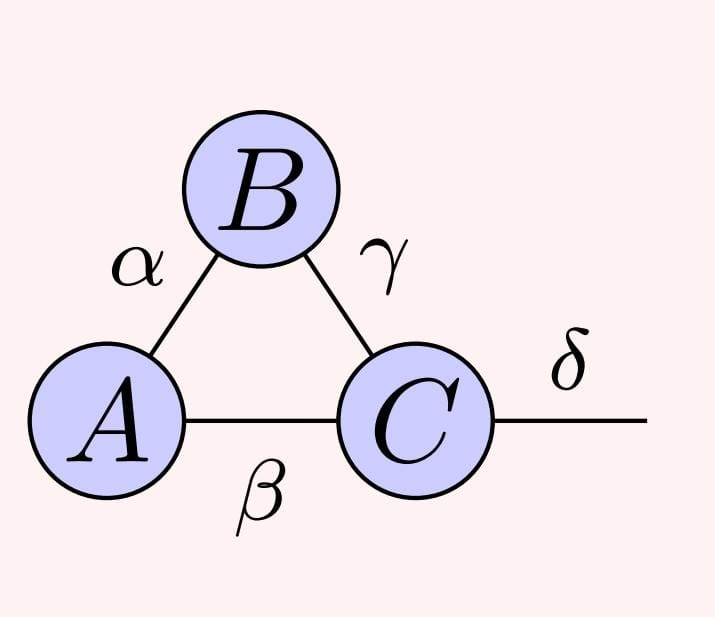
\includegraphics[width=0.2\linewidth]{images/tensorq2-1.jpeg}%
    \caption{The network of Eq.~(1.23), to be bubbled in alphabetical order.}%
\end{figure}


As an example, take the network of Eq.~(1.23): three tensors $A,B,C$ with bonds
$\alpha$ joining $A$ and $B$, $\beta$ joining $A$ and $C$, $\gamma$ joining $B$ and $C$,
and a free leg $\delta$ on $C$. Bubbling in alphabetical order gives


\begin{center}
\begin{tabular}{|c|c|c|c|}
\hline
Current & Tensor & Contract & New \\
\hline
--             & $A$ & --             & $\alpha,\beta$ \\
$\alpha,\beta$ & $B$ & $\alpha$       & $\gamma$ \\
$\beta,\gamma$ & $C$ & $\beta,\gamma$ & $\delta$ \\
\hline
\end{tabular}
\end{center}

Construct the corresponding table for the network of Eq.~(1.24), again bubbling in
alphabetical order.

\begin{figure}[H]\centering
    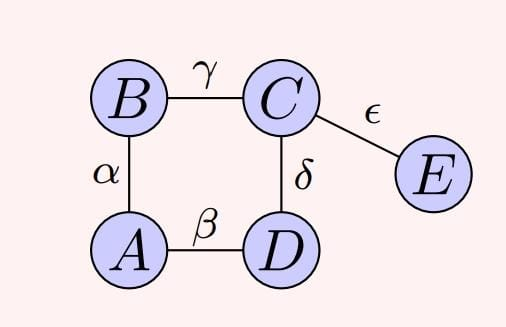
\includegraphics[width=0.2\linewidth]{images/tensorq2-2.jpeg}%
    \caption{The network of Eq.~(1.24), to be bubbled in alphabetical order}%
\end{figure}

and state the largest rank reached by the intermediate object, and whether a different
bubbling order would reduce it.

\end{problem}

% ============================================================== solutions ===

\begin{solution}
.
\vspace{0.1cm}
\begin{center}
\begin{tabular}{|c|c|c|c|}
\hline
Current & Tensor & Contract & New \\
\hline
--                      & $A$ & --          & $\alpha,\beta$ \\
  $\alpha,\beta$        & $B$ & $\alpha$    & $\gamma$   \\
 $\beta,\gamma$         & $C$ &  $\gamma$   &  $\delta,\epsilon$ \\
$\beta,\delta,\epsilon$ & $D$ &   $\delta,\beta$  & -- \\
            $\epsilon$  & $E$ &   $\epsilon$      &  -- \\
\hline
\end{tabular}
\end{center}
\vspace{0.1cm}
The largest rank is achieved after adding the tensor $C$ ($-A-B-C=$), where in this intermediate step we have a $\rank=3$ tensor. We could reduce the highest intermediate rank by starting from $E$, then going to $C$, we would contract $\epsilon$ and the intermediate tensor would be $\rank=2$, then, we can follow the adjacent $\rank=2$ tensors in the orders $B,A,D$ or $D,A,B$, on both cases at least one index is contracted and at most one is added, keeping the $\rank$ always lower or equal to $2$.
\end{solution}



\attempt{
  date        = 2026-09-14,
  time        = 10min,
  difficulty  = 1,
  how it went = ,
}

\end{entry}